% EduConnect - Final Capstone Project Proposal and Prototyping (Part I)
% Overleaf-compatible: upload the whole docs/proposal folder (main.tex, references.bib, figures/, generated/).
% Compile with pdfLaTeX + BibTeX (Overleaf default).
\documentclass[11pt,a4paper]{article}

\usepackage[T1]{fontenc}
\usepackage{lmodern}
\usepackage[utf8]{inputenc}
\usepackage[a4paper,margin=2.4cm]{geometry}
\usepackage{setspace}
\usepackage{microtype}
\usepackage{xcolor}
\usepackage{graphicx}
\usepackage{float}
\usepackage{booktabs}
\usepackage{longtable}
\usepackage{array}
\usepackage{tabularx}
\usepackage{enumitem}
\usepackage{amsmath}
\usepackage{caption}
\usepackage{fancyhdr}
\usepackage{pdflscape}
\usepackage{tikz}
\usepackage{pgfgantt}
\usepackage[hidelinks]{hyperref}
\usepackage{url}

\definecolor{edublue}{HTML}{1F4E79}
\definecolor{placeholder}{HTML}{B42318}
\hypersetup{colorlinks=true,linkcolor=edublue,citecolor=edublue,urlcolor=edublue,
  pdftitle={EduConnect - Smart Student-Tutor Matching System: Capstone Proposal},pdfauthor={[Student Name]}}
\setstretch{1.12}
\emergencystretch=3em
\setlength{\parskip}{0.45em}
\setlength{\parindent}{0pt}
\setlist{itemsep=0.1em,topsep=0.3em}
\captionsetup{font=small,labelfont={bf,color=edublue}}
\graphicspath{{figures/}{docs/proposal/figures/}}
\renewcommand{\arraystretch}{1.18}

% Placeholders the student must replace before submission.
\newcommand{\ph}[1]{\textcolor{placeholder}{\textbf{[#1]}}}
\newcommand{\studentname}{\ph{Student Name}}
\newcommand{\studentid}{\ph{Student ID}}
\newcommand{\coursetitle}{\ph{Course Title}}
\newcommand{\coursecode}{\ph{Course Code}}
\newcommand{\instructor}{\ph{Instructor Name}}
\newcommand{\department}{\ph{Department}}
\newcommand{\submissiondate}{\ph{Submission Date}}

\pagestyle{fancy}
\fancyhf{}
\lhead{\small EduConnect -- Capstone Proposal (Part I)}
\rhead{\small MBSTU}
\cfoot{\small Page \thepage}
\renewcommand{\headrulewidth}{0.4pt}

\newcommand{\figimg}[2][0.95]{\includegraphics[width=#1\linewidth,height=0.82\textheight,keepaspectratio]{#2}}

\begin{document}

%-------------------------------------------------------------------
\begin{titlepage}
\centering
\vspace*{0.6cm}
{\large\bfseries Mawlana Bhashani Science and Technology University (MBSTU)}\\[0.2cm]
{\normalsize Santosh, Tangail, Bangladesh}\\[0.2cm]
{\normalsize \department}\\[1.6cm]
{\color{edublue}\rule{\linewidth}{1.2pt}}\\[0.5cm]
{\Huge\bfseries\color{edublue} EduConnect}\\[0.3cm]
{\Large Smart Student--Tutor Matching System}\\[0.5cm]
{\color{edublue}\rule{\linewidth}{1.2pt}}\\[1.2cm]
{\Large\bfseries Final Capstone Project Proposal and Prototyping}\\[0.2cm]
{\large Part I}\\[1.8cm]
\begin{tabular}{@{}rl@{}}
\textbf{Submitted by:} & \studentname \\
\textbf{Student ID:} & \studentid \\
\textbf{Course Title:} & \coursetitle \\
\textbf{Course Code:} & \coursecode \\
\textbf{Instructor:} & \instructor \\
\textbf{Submission Date:} & \submissiondate \\
\end{tabular}\\[2cm]
{\small Red bracketed items are placeholders to be replaced before submission.}
\vfill
{\small Source repository: \texttt{EduConnect} (see \texttt{README.md}).}
\end{titlepage}

%-------------------------------------------------------------------
\pagenumbering{roman}
\section*{Abstract}
\addcontentsline{toc}{section}{Abstract}
Students in Bangladeshi universities often look for private tutors through word of mouth, social-media groups or notice boards. This process is slow and opaque: students cannot easily compare tutors by subject expertise, price, teaching mode and real availability, and tutors lose students because schedules are coordinated by hand. \textbf{EduConnect} is a web-based system that matches a student's stated requirements (subject, budget, teaching mode, preferred days and time window, minimum rating) to suitable tutors using a transparent weighted-scoring model, shows an explained compatibility score for each tutor, checks live availability, and lets the student request a booking while the system prevents double-booking and overlapping sessions.

This document is the Part I deliverable. It presents the problem, objectives, scope, requirements, feasibility analysis, the chosen process model (incremental development with evolutionary prototyping), an eight-week schedule, system architecture and six UML/structured-analysis diagrams (DFD, use case, activity, ERD, class and object), a risk analysis, a testing plan and the expected outcomes. A working prototype built with HTML, CSS and vanilla JavaScript demonstrates ten classes (plus one enumeration) that also appear in the class diagram, including the weighted matching algorithm, availability checking, conflict-free booking and booking-status display. The report, diagrams, database schema and prototype were designed together so that names, attributes and rules are consistent across all of them.

\medskip
\textbf{Keywords:} tutor matching, recommender system, weighted scoring, booking, UML, prototype, MBSTU.

\newpage
\tableofcontents
\newpage
\listoffigures
\listoftables
\newpage
\pagenumbering{arabic}

%===================================================================
\section{Introduction}
\subsection{Background}
Private tutoring is a widespread complement to formal education in many countries, including Bangladesh \cite{bray2009}. University students commonly seek help in foundational courses such as calculus, data structures, physics and English composition. At the same time, internet access and smartphone use are high enough among young Bangladeshis that a web-based service is a realistic delivery channel \cite{datareportal2024}.

Today, matching is informal: a student posts a request in a Facebook group, collects replies, compares prices by chat and negotiates a time. Each step is manual, information is incomplete, and nobody checks whether the tutor's free time truly fits the student's timetable.

\subsection{Project Overview}
EduConnect is a smart student--tutor matching system. The student enters requirements once; the system filters tutors who teach the subject, scores each candidate on six weighted factors, ranks them, explains every score, and allows the student to request a free slot. A booking moves through the states \emph{Pending}, \emph{Confirmed}, \emph{Completed} or \emph{Cancelled}, and the system refuses any request that would create a double booking.

\subsection{Document Organisation}
Sections 2--6 define the problem, objectives, scope, requirements and feasibility. Section 7 justifies the process model and Section 8 gives the schedule. Section 9 presents the design, Section 10 the prototype, Sections 11--12 the risks and test plan, and Section 13 the expected outcomes.

%===================================================================
\section{Problem Statement}
Students who need academic help face four connected problems:
\begin{enumerate}
  \item \textbf{Discovery:} no single place lists tutors with verified subjects, prices and ratings.
  \item \textbf{Fit:} choosing a tutor means balancing expertise, budget, mode (online or in person), rating and schedule; students do this mentally and inconsistently.
  \item \textbf{Availability:} a tutor who looks perfect may have no free slot at the needed time, which is discovered only after several messages.
  \item \textbf{Coordination:} manual scheduling causes double bookings and overlapping commitments for both students and tutors.
\end{enumerate}
\textbf{Problem to solve:} there is no transparent, availability-aware, conflict-free way for a student to find and book a suitable tutor quickly. EduConnect addresses this gap.

%===================================================================
\section{Objectives}
\subsection{General Objective}
Design and prototype a web system that recommends and books the most suitable tutor for a student's requirements with explainable results and no scheduling conflicts.

\subsection{Specific Objectives}
\begin{table}[H]
\centering
\caption{Specific, measurable objectives}
\begin{tabularx}{\linewidth}{@{}l X X@{}}
\toprule
\textbf{ID} & \textbf{Objective} & \textbf{Measure of success}\\ \midrule
O1 & Capture structured student requirements & Form validates 6 inputs; invalid input blocked with messages\\
O2 & Rank tutors with a weighted model & Six factors, weights sum to 100\%; scores in 0--100\\
O3 & Explain every compatibility score & Per-factor weight, fit and points shown for each tutor\\
O4 & Check tutor availability & Only free slots offered; matching slots highlighted\\
O5 & Prevent booking conflicts & 0 double bookings in conflict test cases (TC09--TC12)\\
O6 & Show booking status & Four states displayed with allowed transitions only\\
O7 & Produce consistent design artefacts & Six diagrams whose names match prototype classes\\
O8 & Deliver in eight weeks & All milestones M1--M6 met (Section~\ref{sec:schedule})\\
\bottomrule
\end{tabularx}
\end{table}

%===================================================================
\section{Scope}
\subsection{In Scope (Part I)}
\begin{itemize}
  \item Complete proposal, six diagrams, database schema and eight-week plan.
  \item Browser-based prototype implementing requirement input, weighted matching with explanations, availability checking, booking with conflict prevention and booking-status display using synthetic data.
  \item Ten JavaScript classes (plus the \texttt{BookingStatus} enumeration) matching the class diagram; automated unit tests for the logic.
\end{itemize}
\subsection{Out of Scope for the Prototype (Planned for the Full System)}
\begin{itemize}
  \item User registration, authentication, administrator verification of tutors and subject management (use cases UC1, UC2, UC11, UC13, UC14).
  \item Server-side database, payments, reviews, chat, push/SMS notifications and mobile apps.
  \item Calendar dates, time zones and recurring-session management.
\end{itemize}
\subsection{Assumptions and Constraints}
\begin{itemize}
  \item Availability is weekly and recurring (Saturday--Thursday working week; Friday is a holiday).
  \item Prices are in Bangladeshi taka (BDT) per hour; ratings are on a 0--5 scale.
  \item One student developer, eight weeks, no paid infrastructure; the stack must run offline in a browser.
\end{itemize}

%===================================================================
\section{Requirements}
\subsection{Stakeholders and User Classes}
\textbf{Student} (searches and books), \textbf{Tutor} (publishes subjects and availability, answers requests), \textbf{Administrator} (verifies tutors, manages subjects), and the \textbf{course instructor/evaluator} (assesses the capstone).

\subsection{Functional Requirements}
Requirements follow the guidance of ISO/IEC/IEEE 29148 \cite{iso29148}. The ``Prototype'' column shows whether Part I implements the requirement.

\begin{table}[H]
\centering
\caption{Functional requirements}
\small
\begin{tabularx}{\linewidth}{@{}l X l l@{}}
\toprule
\textbf{ID} & \textbf{Requirement} & \textbf{Use case} & \textbf{Prototype}\\ \midrule
FR1 & Users shall register and log in with a role (student, tutor, admin). & UC1 & Planned\\
FR2 & Users shall manage their profile data. & UC2 & Planned\\
FR3 & A student shall submit requirements: subject, maximum budget, mode, days, time window, minimum rating. & UC3 & Yes\\
FR4 & The system shall rank tutors who teach the subject by a weighted compatibility score (0--100). & UC4 & Yes\\
FR5 & The system shall explain each score by factor, weight and points. & UC5 & Yes\\
FR6 & The system shall check tutor availability and highlight free slots matching the request. & UC6 & Yes\\
FR7 & A student shall request a booking for a free slot. & UC7 & Yes\\
FR8 & The system shall reject a booking if the slot is taken or overlaps another active booking of the student or tutor. & UC8 & Yes\\
FR9 & The system shall display booking status (Pending, Confirmed, Completed, Cancelled). & UC9 & Yes\\
FR10 & A student shall cancel a pending or confirmed booking, releasing the slot. & UC10 & Yes\\
FR11 & A tutor shall manage availability slots. & UC11 & Seed data\\
FR12 & A tutor shall accept, decline or complete a booking. & UC12 & Simulated\\
FR13 & An administrator shall verify tutor profiles. & UC13 & Planned\\
FR14 & An administrator shall manage the subject catalogue. & UC14 & Planned\\
\bottomrule
\end{tabularx}
\end{table}

\subsection{Non-Functional Requirements}
Quality attributes are drawn from ISO/IEC 25010 \cite{iso25010}.
\begin{table}[H]
\centering
\caption{Non-functional requirements}
\small
\begin{tabularx}{\linewidth}{@{}l l X@{}}
\toprule
\textbf{ID} & \textbf{Attribute} & \textbf{Requirement}\\ \midrule
NFR1 & Usability & Responsive from 360\,px phones to desktops; keyboard-operable controls; target WCAG 2.1 AA contrast and labels \cite{wcag21}; follows common usability heuristics \cite{nielsen1994}.\\
NFR2 & Performance & Ranking of up to 1\,000 tutors in under one second on a typical laptop (to be measured in system testing).\\
NFR3 & Reliability / integrity & No double booking: enforced in application logic and, in the full system, by a database partial unique index.\\
NFR4 & Security & Hashed passwords, HTTPS, server-side validation and role-based access (full system).\\
NFR5 & Maintainability & Modular classes, one responsibility per file, automated unit tests for core logic.\\
NFR6 & Portability & Runs in current Chrome, Firefox, Edge and Safari without build tools.\\
NFR7 & Explainability & Every ranking decision is decomposable into factor-level points shown to the user.\\
\bottomrule
\end{tabularx}
\end{table}

%===================================================================
\section{Feasibility Analysis}
\subsection{Technical Feasibility}
The prototype uses only standard web technologies (HTML5, CSS3, ECMAScript classes \cite{ecma262}). The weighted-sum model is a well-established multi-criteria decision method \cite{triantaphyllou2000} and a common baseline in recommender systems \cite{ricci2022}. All algorithms are $O(n)$ per request over $n$ candidate tutors, so a browser handles realistic data volumes. The full system can use any open-source relational database and web framework. \textbf{Verdict: feasible.}

\subsection{Economic Feasibility}
\begin{table}[H]
\centering
\caption{Illustrative cost estimate (assumptions, not quotations)}
\small
\begin{tabularx}{\linewidth}{@{}X l X@{}}
\toprule
\textbf{Item} & \textbf{Estimate} & \textbf{Note}\\ \midrule
Development tools (VS Code, Git, Node.js, PlantUML, TeX) & 0 BDT & Free and open source\\
Prototype hosting (GitHub Pages) & 0 BDT & Static site\\
Internet data for 8 weeks & \ph{amount} BDT & Student's existing plan\\
Developer effort & $\approx$120 hours & Student time, not charged\\
Printing and binding of report & \ph{amount} BDT & If a hard copy is required\\
Full-system VPS (future) & $\approx$ \ph{amount} BDT/month & Low-tier virtual server\\
\bottomrule
\end{tabularx}
\end{table}
Since the prototype needs no paid resources, Part I is economically feasible. A future deployment could be funded by a small booking commission or sponsorship; this is outside Part I.

\subsection{Operational Feasibility}
Students already use web forms and messaging apps, so the interaction (fill a form, read a ranked list, click a slot) is familiar. Tutors need only to publish subjects and weekly availability. Because rankings are explained, users can judge the recommendation rather than trust a black box.

\subsection{Schedule Feasibility}
The scope is deliberately limited to a prototype with synthetic data. Section~\ref{sec:schedule} breaks the work into 13 tasks with finish-to-start dependencies, which fit within eight weeks with one week of final review.

\subsection{Legal, Ethical and Social Feasibility}
The prototype stores no real personal data. A production system must comply with applicable Bangladeshi data-protection and ICT law, obtain consent for personal data, avoid discriminatory ranking (for example, new tutors without ratings must not be permanently hidden), and keep tutor verification transparent.

%===================================================================
\section{Software Process Model}
\subsection{Candidate Models}
\begin{table}[H]
\centering
\caption{Comparison of candidate process models for this project}
\small
\begin{tabularx}{\linewidth}{@{}l X X X@{}}
\toprule
\textbf{Model} & \textbf{Strengths} & \textbf{Weaknesses here} & \textbf{Fit}\\ \midrule
Waterfall \cite{sommerville2016} & Clear phases, easy documentation & Late feedback; changes are costly; prototype arrives last & Low\\
Spiral \cite{boehm1988} & Strong risk management & Heavy overhead for one developer and 8 weeks & Medium\\
Scrum / Agile \cite{agile2001,scrumguide2020} & Short iterations, frequent feedback & Full ceremonies are too heavy for one person & Medium\\
\textbf{Incremental + evolutionary prototyping} \cite{pressman2020} & Working increments, early demos, lightweight & Needs discipline in documentation & \textbf{High}\\
\bottomrule
\end{tabularx}
\end{table}

\subsection{Chosen Model and Justification}
EduConnect uses the \textbf{incremental model with evolutionary prototyping}, organised in one-week sprints borrowed from Scrum (a short plan, a working increment, a short review). The reasons are:
\begin{enumerate}
  \item \textbf{Deliverable is a prototype:} the assignment explicitly requires a working prototype, so a model that produces runnable increments early is natural.
  \item \textbf{Time-boxed:} eight fixed weeks suit fixed-length sprints with a milestone at the end of each increment.
  \item \textbf{Moderately stable but refinable requirements:} the core features are known, but weights, input fields and the explanation format benefit from feedback after each increment.
  \item \textbf{Risk reduction:} the riskiest parts (matching quality and conflict-free booking) are built and tested first (increment 3), not at the end.
  \item \textbf{Small team:} one developer cannot sustain full Scrum roles, but can run the lightweight cycle of plan, build, test and review.
\end{enumerate}

\begin{table}[H]
\centering
\caption{Increments and their mapping to weeks}
\small
\begin{tabularx}{\linewidth}{@{}l l X X@{}}
\toprule
\textbf{Increment} & \textbf{Weeks} & \textbf{Content} & \textbf{Output}\\ \midrule
1 & 1--2 & Requirements, literature, SRS, use cases, ERD & Baseline (M1)\\
2 & 3 & DFD, activity, class and object models; wireframes & Design complete (M2)\\
3 & 4--5 & Matching algorithm; availability and booking logic & Tested core logic (M3)\\
4 & 6--7 & UI integration, status display, testing & Integrated prototype (M4), tested (M5)\\
5 & 8 & Final review, packaging, submission & Submission (M6)\\
\bottomrule
\end{tabularx}
\end{table}

%===================================================================
\section{Project Schedule}\label{sec:schedule}
The plan below is generated from \texttt{docs/schedule/tasks.csv} so that the chart and tables stay consistent. All dependencies are finish-to-start, and every task starts in a later week than its predecessors end.

\begin{landscape}
\begin{figure}[H]
\centering
\resizebox{!}{0.68\textheight}{\begin{ganttchart}[hgrid, vgrid={*{8}{draw=gray!30}}, y unit title=0.55cm, y unit chart=0.5cm, x unit=0.9cm,
  title height=1, bar height=0.55, bar/.append style={fill=blue!45!black}, milestone/.append style={fill=orange!80!black},
  bar label font=\scriptsize, milestone label font=\scriptsize, title label font=\scriptsize, link/.style={->, gray}]{1}{8}
\gantttitle{Project week}{8} \\
\gantttitlelist{1,...,8}{1} \\
\ganttbar[name=T1]{T1 Requirements elicitation and stakeholder survey}{1}{1} \\
\ganttbar[name=T2]{T2 Related-system review and literature search}{1}{2} \\
\ganttbar[name=T3]{T3 SRS and use-case modelling}{2}{2} \\
\ganttbar[name=T4]{T4 Database and data modelling}{2}{2} \\
\ganttbar[name=T5]{T5 Process modelling (DFD and activity)}{3}{3} \\
\ganttbar[name=T6]{T6 Class and object modelling}{3}{3} \\
\ganttbar[name=T7]{T7 UI wireframes and responsive layout}{3}{4} \\
\ganttbar[name=T8]{T8 Matching algorithm implementation}{4}{5} \\
\ganttbar[name=T9]{T9 Availability and booking module}{4}{5} \\
\ganttbar[name=T10]{T10 UI integration and status display}{6}{6} \\
\ganttbar[name=T11]{T11 Testing and defect fixing}{7}{7} \\
\ganttbar[name=T12]{T12 Proposal writing and review}{3}{7} \\
\ganttbar[name=T13]{T13 Final review packaging and submission}{8}{8} \\
\ganttmilestone[name=M1]{M1 Requirements baseline (SRS approved)}{2} \\
\ganttmilestone[name=M2]{M2 Design complete (six diagrams)}{3} \\
\ganttmilestone[name=M3]{M3 Core logic complete (matcher + booking)}{5} \\
\ganttmilestone[name=M4]{M4 Integrated prototype}{6} \\
\ganttmilestone[name=M5]{M5 Testing complete}{7} \\
\ganttmilestone[name=M6]{M6 Final submission}{8}
\ganttlink{T1}{T3}
\ganttlink{T1}{T4}
\ganttlink{T3}{T5}
\ganttlink{T3}{T6}
\ganttlink{T4}{T6}
\ganttlink{T3}{T7}
\ganttlink{T6}{T8}
\ganttlink{T6}{T9}
\ganttlink{T7}{T10}
\ganttlink{T8}{T10}
\ganttlink{T9}{T10}
\ganttlink{T10}{T11}
\ganttlink{T3}{T12}
\ganttlink{T11}{T13}
\ganttlink{T12}{T13}
\end{ganttchart}
}
\caption{Eight-week Gantt chart with dependencies and milestones}
\label{fig:gantt}
\end{figure}
\end{landscape}

\begin{table}[H]
\centering
\caption{Task list with dependencies and deliverables}
\small
\begin{longtable}{@{}p{0.6cm}p{4.6cm}c p{1.8cm} p{4.6cm}@{}}
\toprule
\textbf{ID} & \textbf{Task} & \textbf{Weeks} & \textbf{Depends on} & \textbf{Deliverable} \\ \midrule \endhead
T1 & Requirements elicitation and stakeholder survey & 1 & -- & Requirement notes; survey summary \\
T2 & Related-system review and literature search & 1--2 & -- & Literature summary; reference list \\
T3 & SRS and use-case modelling & 2 & T1 & SRS draft; Use Case Diagram \\
T4 & Database and data modelling & 2 & T1 & ERD; relational schema \\
T5 & Process modelling (DFD and activity) & 3 & T3 & DFD (L0/L1); Activity Diagram \\
T6 & Class and object modelling & 3 & T3,T4 & Class Diagram; Object Diagram \\
T7 & UI wireframes and responsive layout & 3--4 & T3 & Wireframes; CSS foundation \\
T8 & Matching algorithm implementation & 4--5 & T6 & matcher.js; unit tests \\
T9 & Availability and booking module & 4--5 & T6 & bookingManager.js; conflict tests \\
T10 & UI integration and status display & 6 & T7,T8,T9 & Integrated prototype \\
T11 & Testing and defect fixing & 7 & T10 & Test results; testing checklist \\
T12 & Proposal writing and review & 3--7 & T3 & main.tex; proposal PDF \\
T13 & Final review packaging and submission & 8 & T11,T12 & GitHub repository; ZIP \\
\bottomrule
\end{longtable}

\end{table}

\begin{table}[H]
\centering
\caption{Milestones}
\small
\begin{tabular}{@{}p{5.4cm}c p{2cm} p{4cm}@{}}
\toprule
\textbf{Milestone} & \textbf{Week} & \textbf{Gate task} & \textbf{Exit criterion} \\ \midrule
M1 Requirements baseline (SRS approved) & 2 & T3,T4 & SRS signed off \\
M2 Design complete (six diagrams) & 3 & T5,T6 & All six diagrams reviewed \\
M3 Core logic complete (matcher + booking) & 5 & T8,T9 & Unit tests pass \\
M4 Integrated prototype & 6 & T10 & Demo scenario runs end to end \\
M5 Testing complete & 7 & T11 & Checklist signed off \\
M6 Final submission & 8 & T13 & Submitted package \\
\bottomrule
\end{tabular}

\end{table}

%===================================================================
\section{System Design}
\subsection{Architecture}
The full system follows a three-tier architecture (Figure~\ref{fig:arch}): a responsive browser UI, an application tier with matching, booking, availability, authentication and notification services, and a relational database. The Part I prototype implements the highlighted components in the browser and stores bookings in \texttt{localStorage}.
\begin{figure}[H]\centering\figimg[0.9]{architecture.png}\caption{System architecture (green = implemented in the prototype)}\label{fig:arch}\end{figure}

\subsection{Data Flow Diagram}
Figure~\ref{fig:dfd0} shows the context (Level 0) and Figure~\ref{fig:dfd1} the Level 1 decomposition into six processes (accounts, requirements, matching, availability, booking and status update) and five data stores. Data store D3 is shared by matching, availability and booking, which is where conflicts are detected.
\begin{figure}[H]\centering\figimg[0.95]{dfd_level0.png}\caption{DFD Level 0 -- context diagram}\label{fig:dfd0}\end{figure}
\begin{landscape}
\begin{figure}[H]\centering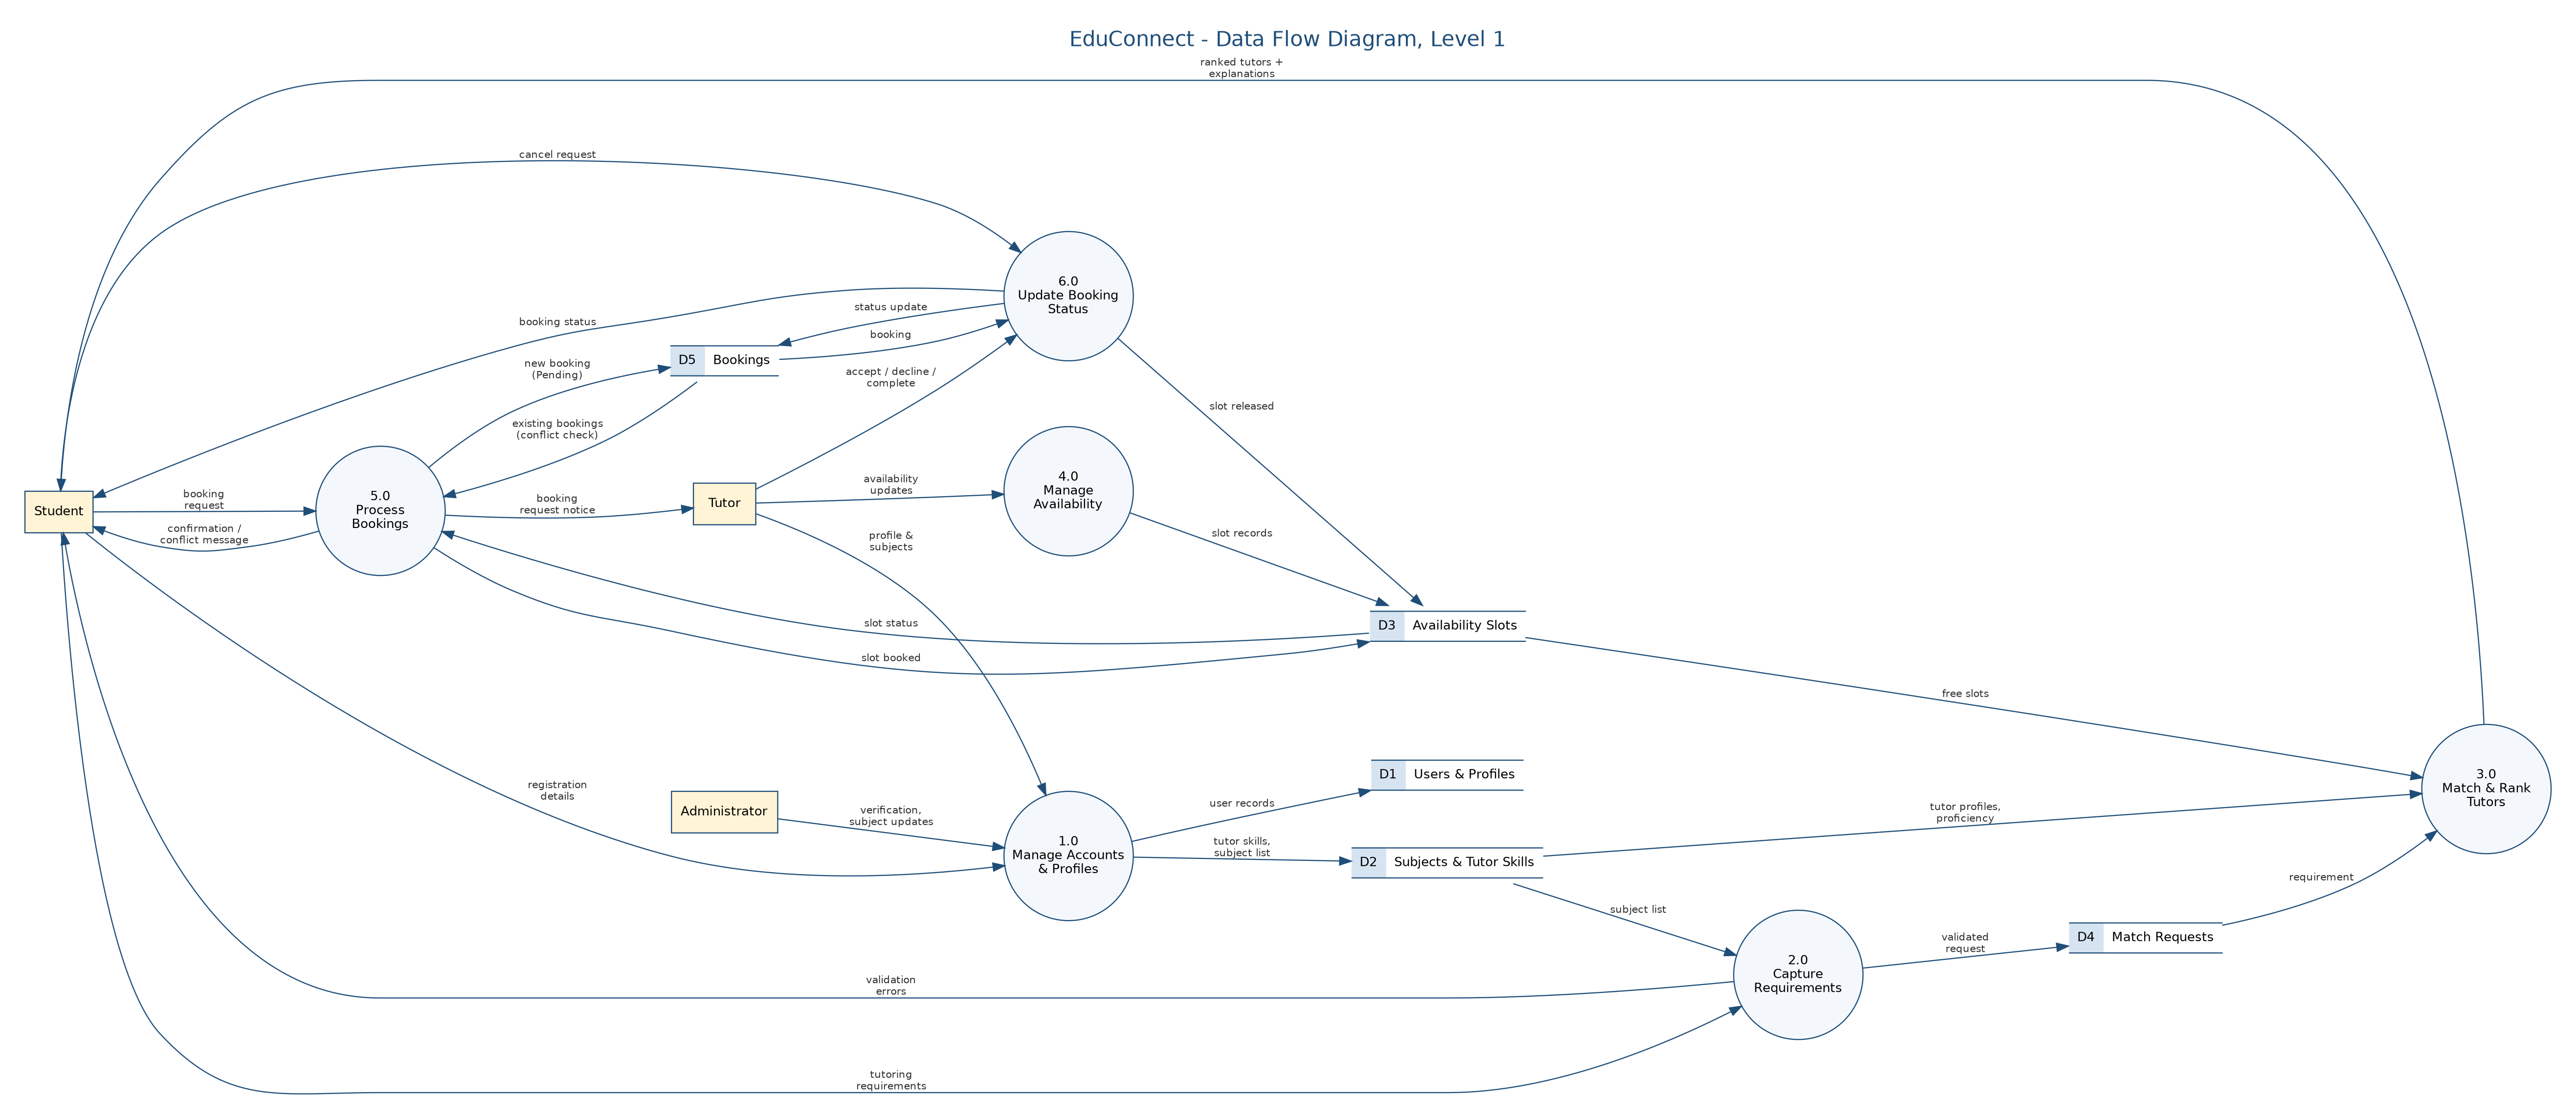
\includegraphics[width=0.96\linewidth,height=0.78\textheight,keepaspectratio]{dfd_level1.png}\caption{DFD Level 1}\label{fig:dfd1}\end{figure}
\end{landscape}

\subsection{Use Case Diagram}
Fourteen use cases are defined for three actors (Figure~\ref{fig:uc}). \emph{View Ranked Tutor Matches} includes submitting requirements, explaining scores and checking availability; \emph{Book Session} includes conflict prevention.
\begin{figure}[H]\centering\figimg[0.95]{usecase.png}\caption{Use case diagram}\label{fig:uc}\end{figure}

\subsection{Activity Diagram}
Figure~\ref{fig:act} models the main scenario with three swim-lanes (Student, System, Tutor), including input validation, ranking, the conflict check and the tutor's response.
\begin{figure}[H]\centering\figimg[0.8]{activity.png}\caption{Activity diagram: match and book a tutor}\label{fig:act}\end{figure}

\subsection{Entity Relationship Diagram and Database Schema}
The ERD (Figure~\ref{fig:erd}) has eight entities. Users have a role and an optional student or tutor profile; tutors teach subjects with a proficiency (1--5) through the associative entity \texttt{tutor\_subjects}; tutors offer availability slots; students submit match requests and make bookings. The business rule ``at most one active booking per slot'' is enforced by a partial unique index in \texttt{database/schema.sql}, which was tested with SQLite (\texttt{tests/test\_schema.py}). The design follows standard relational modelling practice \cite{elmasri2016}.
\begin{figure}[H]\centering\figimg[0.95]{erd.png}\caption{Entity relationship diagram (crow's foot notation)}\label{fig:erd}\end{figure}

\subsection{Class Diagram}
The class diagram (Figure~\ref{fig:class}) contains the ten classes and one enumeration implemented in the prototype. \texttt{Student} and \texttt{Tutor} specialise \texttt{User}; \texttt{Tutor} composes \texttt{AvailabilitySlot}; \texttt{TutorMatcher} produces \texttt{MatchResult}; \texttt{BookingManager} aggregates \texttt{Booking}. Notation follows UML \cite{fowler2003}.
\begin{figure}[H]\centering\figimg[0.98]{class.png}\caption{Class diagram}\label{fig:class}\end{figure}

\subsection{Object Diagram}
Figure~\ref{fig:obj} is a snapshot of the demo scenario: student Nusrat Jahan asks for Data Structures online, at most 650~BDT/h, on Saturday or Monday between 18:00 and 20:00; the matcher returns Rahim Uddin first with a score of 93.2, and booking B002 is created in the \emph{Pending} state.
\begin{figure}[H]\centering\figimg[0.98]{object.png}\caption{Object diagram of the demo scenario}\label{fig:obj}\end{figure}

\subsection{Matching Algorithm}
A tutor is a candidate only if verified and teaching the requested subject. For each candidate, six component scores $c_i\in[0,1]$ are combined with weights $w_i$ \cite{triantaphyllou2000}:
\[
\text{Score} = 100\cdot\frac{\sum_{i=1}^{6} w_i\,c_i}{\sum_{i=1}^{6} w_i}
\]
\begin{table}[H]
\centering
\caption{Scoring components (default weights sum to 100)}
\small
\begin{tabularx}{\linewidth}{@{}l c X@{}}
\toprule
\textbf{Component} & \textbf{Weight} & \textbf{Component score $c_i$}\\ \midrule
Subject expertise & 30 & proficiency\,/\,5\\
Availability fit & 25 & With a time window: best overlap of a free slot (on requested days) divided by window length. Without: $\min(1,\text{free slots}/3)$.\\
Budget fit & 15 & Rate $\le$ budget: $1-0.3\cdot$rate/budget (0.7--1.0). Over budget: $\max(0,\,0.7-(\text{rate}-\text{budget})/\text{budget})$.\\
Rating & 15 & rating\,/\,5, halved if below the student's minimum rating\\
Teaching mode & 10 & 1 if student has no preference, tutor teaches both, or modes equal; else 0\\
Experience & 5 & $\min(\text{years}/5,\,1)$\\
\bottomrule
\end{tabularx}
\end{table}
Ties are broken by rating (higher first) and then rate (lower first). Table~\ref{tab:worked} shows the worked example from the object diagram, reproduced by the prototype and its unit tests.
\begin{table}[H]
\centering
\caption{Worked example: Rahim Uddin (T001) for the demo requirement}\label{tab:worked}
\small
\begin{tabular}{@{}lccc@{}}
\toprule
\textbf{Factor} & \textbf{Weight} & \textbf{Fit} & \textbf{Points}\\ \midrule
Subject expertise (5/5) & 30\% & 100\% & 30.0\\
Availability (2 slots cover window) & 25\% & 100\% & 25.0\\
Budget (600 vs 650 BDT/h) & 15\% & 72\% & 10.8\\
Rating (4.8/5) & 15\% & 96\% & 14.4\\
Mode (Online = Online) & 10\% & 100\% & 10.0\\
Experience (3 years) & 5\% & 60\% & 3.0\\ \midrule
\textbf{Total} & 100\% & & \textbf{93.2}\\
\bottomrule
\end{tabular}
\end{table}

%===================================================================
\section{Prototype}
\subsection{Implemented Features}
The prototype (\texttt{prototype/index.html}) is a responsive single-page interface that runs from a local file or any static host with no build step.
\begin{itemize}
  \item \textbf{Requirement input} with validation (FR3).
  \item \textbf{Weighted ranking} with adjustable priorities, a score bar and a ``Why this score?'' table (FR4, FR5).
  \item \textbf{Availability checking:} free slots highlighted when they fit the requested days and time window; booked slots are disabled (FR6).
  \item \textbf{Booking and conflict prevention:} slot already taken, tutor overlap and student overlap are rejected with an explanation (FR7, FR8).
  \item \textbf{Booking status display} with simulated tutor actions and student cancellation (FR9, FR10, FR12).
\end{itemize}

\subsection{Class-to-File Mapping}
\begin{table}[H]
\centering
\caption{Classes in the class diagram and their implementation}
\small
\begin{tabularx}{\linewidth}{@{}l l X@{}}
\toprule
\textbf{Class} & \textbf{File} & \textbf{Responsibility}\\ \midrule
User, Student, Tutor & \texttt{js/models.js} & People; tutor holds proficiency map and slots\\
Subject & \texttt{js/models.js} & Course catalogue entry\\
AvailabilitySlot & \texttt{js/models.js} & Weekly slot, overlap maths, book/release\\
StudentRequirement & \texttt{js/models.js} & Requirement data and validation\\
MatchResult, TutorMatcher & \texttt{js/matcher.js} & Scoring, ranking, explanations\\
Booking, BookingManager & \texttt{js/bookingManager.js} & Status lifecycle, conflict detection, persistence\\
\bottomrule
\end{tabularx}
\end{table}

\subsection{Limitations}
The prototype has no server, authentication or real database; data are synthetic; slots are recurring weekly without dates; tutor responses are simulated; weights are hand-chosen and not learned; and client-side conflict checks must be repeated server-side in a production system. These are stated in the user interface and in the README.

\subsection{How to Run}
Open \texttt{prototype/index.html} in a browser, or run \texttt{python3 -m http.server} in the \texttt{prototype} folder. Run \texttt{node tests/run-tests.js} for the logic tests.

%===================================================================
\section{Risk Analysis}
Probability (P) and impact (I) are rated Low (L), Medium (M) or High (H).
\begin{table}[H]
\centering
\caption{Risk register}
\small
\begin{tabularx}{\linewidth}{@{}l X c c X@{}}
\toprule
\textbf{ID} & \textbf{Risk} & \textbf{P} & \textbf{I} & \textbf{Mitigation / contingency}\\ \midrule
R1 & Requirement creep during prototyping & M & H & Freeze scope at M1; log new ideas as ``future work''\\
R2 & Schedule slip (illness, exams, load-shedding) & M & H & One-week buffer in week 8; work offline; Git commits daily\\
R3 & Poor or biased ranking (e.g.\ new tutors disadvantaged) & M & M & Transparent scores; adjustable weights; neutral rating default planned for tutors without reviews\\
R4 & Double booking in production due to concurrent requests & M & H & Database partial unique index and transactions (schema tested)\\
R5 & Cold start: too few tutors or ratings & H & M & Seed data in prototype; admin-assisted onboarding in full system\\
R6 & Privacy or misuse of personal data & M & H & Collect minimum data; hash passwords; consent and retention policy\\
R7 & Browser storage unavailable or corrupted & L & L & Prototype falls back to in-memory seed data\\
R8 & Loss of work or file corruption & L & H & Git repository, remote backup, ZIP snapshot at each milestone\\
R9 & Inconsistency between report, diagrams and code & M & M & Single class list; consistency checks listed in the test plan\\
\bottomrule
\end{tabularx}
\end{table}

%===================================================================
\section{Testing Plan}
\subsection{Strategy}
Testing follows the usual levels \cite{myers2011}: unit tests for model, matcher and booking logic (\texttt{tests/run-tests.js}); a schema test (\texttt{tests/test\_schema.py}); integration and system testing through the manual checklist (\texttt{docs/TESTING\_CHECKLIST.md}); usability review against heuristics \cite{nielsen1994}; and acceptance testing against requirements FR3--FR10. Exit criteria: all automated tests pass, no open high-severity defect, and every checklist item for FR3--FR10 passes.

\subsection{Representative Test Cases}
\begin{table}[H]
\centering
\caption{Representative test cases (full list in the repository checklist)}
\small
\begin{tabularx}{\linewidth}{@{}l l X X@{}}
\toprule
\textbf{ID} & \textbf{Req.} & \textbf{Test} & \textbf{Expected result}\\ \midrule
TC01 & FR3 & Submit empty subject or negative budget & Inline errors; no search\\
TC02 & FR3 & Window end earlier than start & Validation error\\
TC03 & FR4 & Demo scenario (Data Structures) & Only T001, T002, T006 listed; T001 first\\
TC04 & FR4 & Scores sorted, within 0--100 & Descending order; all in range\\
TC05 & FR5 & Open ``Why this score?'' & Six factors; points sum to total\\
TC06 & FR6 & Tutor with no free slot on chosen days & Availability fit 0\%\\
TC07 & FR4 & Change weights (e.g.\ budget only) & Ranking changes; all-zero weights rejected\\
TC08 & FR7 & Book a free slot & Booking Pending; slot disabled\\
TC09 & FR8 & Second student books same slot & Rejected: slot taken\\
TC10 & FR8 & Same student books overlapping slots with two tutors & Rejected: overlap\\
TC11 & FR8 & Tutor not teaching the subject & Rejected\\
TC12 & FR8 & Booking persists after page reload & Still listed; slot still blocked\\
TC13 & FR9 & Pending $\rightarrow$ Confirmed $\rightarrow$ Completed & Statuses update; illegal jumps rejected\\
TC14 & FR10 & Cancel booking & Status Cancelled; slot re-bookable\\
TC15 & NFR1 & View on 360\,px width & No horizontal page scroll; controls usable\\
TC16 & NFR3 & Insert two active bookings for one slot in SQL & Second insert rejected\\
\bottomrule
\end{tabularx}
\end{table}

%===================================================================
\section{Expected Outcomes}
\begin{enumerate}
  \item A reviewed proposal that defines problem, scope, requirements, feasibility, process, schedule, risks and tests.
  \item Six consistent diagrams plus architecture and DFD Level 0, each with editable source (PlantUML and Graphviz).
  \item A relational schema consistent with the ERD and verified for double-booking prevention.
  \item A working prototype demonstrating explainable ranking and conflict-free booking, with automated tests (19 logic tests and 5 schema checks).
  \item A professional GitHub repository with README, setup instructions and a ZIP archive for submission.
  \item A foundation for the full system: authentication, server-side persistence, notifications, reviews and learned weights.
\end{enumerate}

\section{Conclusion}
EduConnect turns an informal, error-prone search into a structured and explainable process. The proposal shows that the idea is feasible within eight weeks, that the design artefacts are mutually consistent, and that the prototype already demonstrates the most valuable behaviour: ranking tutors fairly and refusing conflicting bookings.

%===================================================================
\clearpage
\bibliographystyle{ieeetr}
\addcontentsline{toc}{section}{References}
\bibliography{references}

\appendix
\section{Requirement Traceability}
\begin{table}[H]
\centering
\caption{Traceability from requirements to design, code and tests}
\small
\begin{tabularx}{\linewidth}{@{}l l X l@{}}
\toprule
\textbf{Req.} & \textbf{Diagram element} & \textbf{Code} & \textbf{Tests}\\ \midrule
FR3 & UC3; \texttt{StudentRequirement}; \texttt{match\_requests} & \texttt{models.js}, \texttt{app.js} & TC01, TC02\\
FR4, FR5 & UC4, UC5; \texttt{TutorMatcher}, \texttt{MatchResult} & \texttt{matcher.js} & TC03--TC05, TC07\\
FR6 & UC6; \texttt{AvailabilitySlot} & \texttt{models.js}, \texttt{matcher.js} & TC06\\
FR7, FR8 & UC7, UC8; \texttt{BookingManager}; \texttt{bookings} & \texttt{bookingManager.js} & TC08--TC12, TC16\\
FR9, FR10 & UC9, UC10; \texttt{BookingStatus} & \texttt{bookingManager.js}, \texttt{app.js} & TC13, TC14\\
NFR1 & -- & \texttt{styles.css} & TC15\\
\bottomrule
\end{tabularx}
\end{table}

\end{document}
